% Презентация к отчёту по преддипломной практике.
% Объединяет результаты 1 и 2 семестров: сервер + веб-панель + мобильное приложение.
\documentclass[aspectratio=169,12pt]{beamer}

\usepackage[T2A]{fontenc}
\usepackage[utf8]{inputenc}
\usepackage[russian]{babel}
\usepackage{array}
\usepackage{graphicx}
\usepackage{tikz}
\usepackage{xcolor}

\definecolor{mintbg}{RGB}{208,229,205}
\definecolor{mintbgdark}{RGB}{191,221,186}
\definecolor{mintline}{RGB}{148,180,144}
\definecolor{shadowgray}{RGB}{120,120,120}
\definecolor{posblue}{RGB}{84,145,204}
\definecolor{dobrodelorange}{RGB}{230,151,67}
\definecolor{fixgreen}{RGB}{96,167,112}
\definecolor{ourspurple}{RGB}{181,103,181}

\setbeamertemplate{navigation symbols}{}
\setbeamercolor{normal text}{fg=black,bg=white}
\setbeamercolor{title}{fg=black,bg=mintbg}
\setbeamercolor{subtitle}{fg=black,bg=mintbg}
\setbeamercolor{frametitle}{fg=black,bg=mintbg}
\setbeamerfont{frametitle}{size=\Large}
\setbeamerfont{title}{size=\Large}
\setbeamerfont{subtitle}{size=\large}
\setbeamerfont{footline}{size=\small}
\setbeamersize{text margin left=10mm,text margin right=10mm}
\setbeamertemplate{frametitle}{}

\newcommand{\myStudentShortName}{Березкина Е.В.}
\newcommand{\myStudentGroup}{ПИб-4301-01-00}
\newcommand{\myCity}{Киров}
\newcommand{\myYear}{2026}

\title[Программная система фиксации городских событий]{Разработка программной системы\\фиксации городских событий}
\subtitle{Отчёт по преддипломной практике}
\author[\myStudentShortName]{\myStudentShortName}
\date{\myCity, \myYear}

\newcommand{\PresentationDepartmentLine}{Кафедра ЭВМ, ВятГУ}
\newcommand{\PresentationGroupLine}{Группа: \myStudentGroup}
\newcommand{\PresentationShortTitle}{Программная система фиксации городских событий}

% Путь к изображениям из results
\graphicspath{
  {../../results/img/}
  {../../results/img/bpwin/}
  {../../results/img/plantuml/}
  {../../results/img/screenshots/web/}
  {../../results/img/screenshots/mobile/}
  {../../results/img/tests/}
  {img/}
}

\setbeamertemplate{headline}{%
    \ifnum\insertframenumber>1
        \begin{beamercolorbox}[wd=\paperwidth,ht=9mm,dp=1.2mm,leftskip=10mm]{frametitle}
            \usebeamerfont{frametitle}\insertframetitle
        \end{beamercolorbox}
        \vspace{-0.3mm}
        \hbox to \paperwidth{\color{shadowgray}\rule{\paperwidth}{0.4mm}}
    \fi
}

% Футер на полную ширину слайда
\setbeamertemplate{footline}{%
    \nointerlineskip
    \begin{beamercolorbox}[wd=\paperwidth,ht=5.5mm,dp=0mm]{normal text}%
        \begin{tikzpicture}[baseline=0]
            \fill[mintbg] (0,0) rectangle (\paperwidth,5.5mm);
            \draw[line width=0.2mm,black] (.5\paperwidth,0.8mm) -- (.5\paperwidth,4.7mm);
            \node[anchor=center,font=\fontsize{9}{10}\selectfont] at (.25\paperwidth,2.75mm) {\insertshortauthor};
            \node[anchor=center,font=\fontsize{8.6}{9.4}\selectfont,text width=.48\paperwidth,align=center] at (.75\paperwidth,2.75mm) {\PresentationShortTitle};
        \end{tikzpicture}%
    \end{beamercolorbox}%
}

\begin{document}

% ========== Слайд 1: Титульный ==========
\begin{frame}
    \begin{tikzpicture}[remember picture,overlay]
        \fill[rounded corners=2.5mm,shadowgray!55] ([xshift=-0.39\paperwidth+1.6mm,yshift=-0.9cm-1.6mm]current page.north)
            rectangle ([xshift=0.39\paperwidth+1.6mm,yshift=-3.45cm-1.6mm]current page.north);
        \fill[rounded corners=2.5mm,mintbg] ([xshift=-0.39\paperwidth,yshift=-0.9cm]current page.north)
            rectangle ([xshift=0.39\paperwidth,yshift=-3.45cm]current page.north);

        \node[align=center,text width=0.72\paperwidth,font=\fontsize{20}{24}\selectfont] at ([yshift=-1.85cm]current page.north) {\inserttitle};
        \node[align=center,font=\fontsize{17}{20}\selectfont] at ([yshift=-3.0cm]current page.north) {\insertsubtitle};

        \node[align=center,font=\fontsize{20}{24}\selectfont] at ([yshift=-5.4cm]current page.north) {\myStudentShortName};
        \node[align=center,font=\fontsize{15}{18}\selectfont] at ([yshift=-6.45cm]current page.north) {\PresentationGroupLine};
        \node[align=center,font=\fontsize{14}{17}\selectfont] at ([yshift=-7.45cm]current page.north) {\PresentationDepartmentLine};
        \node[align=center,font=\fontsize{16}{19}\selectfont] at ([yshift=-8.05cm]current page.north) {\myYear};
    \end{tikzpicture}
\end{frame}

% ========== Слайд 2: Анализ текущей проблемы ==========
\begin{frame}[c]{Анализ текущей проблемы}
    \begin{columns}[c,totalwidth=\textwidth]
        \begin{column}{0.5\textwidth}
            \footnotesize
            \begin{itemize}\setlength\itemsep{0.45em}
                \item Информация о проблемах поступает по телефону, почте и в личных сообщениях.
                \item Разрозненные каналы приводят к потере обращений.
                \item Нет единого инструмента контроля статусов в реальном времени.
                \item Без интерактивной карты диспетчер не видит общую картину проблем города.
                \item У жителей нет мобильного приложения для фиксации проблем на месте.
            \end{itemize}
        \end{column}
        \begin{column}{0.5\textwidth}
            \centering
            \includegraphics[width=0.9\linewidth,height=0.78\textheight,keepaspectratio]{current_a-0.png}
        \end{column}
    \end{columns}
\end{frame}

% ========== Слайд 3: Цель и задачи работы ==========
\begin{frame}[c]{Цель и задачи работы}
    \begin{columns}[c,totalwidth=\textwidth]
        \begin{column}{0.42\textwidth}
            \scriptsize
            \textbf{Цель:} разработать программную систему для фиксации и обработки обращений о проблемах городской инфраструктуры.

            \vspace{0.45em}
            \textbf{Задачи:}
            \begin{itemize}\setlength\itemsep{0.15em}
                \item провести анализ предметной области;
                \item спроектировать структуру системы и базу данных;
                \item реализовать серверную часть с API;
                \item разработать веб-панель диспетчера;
                \item создать мобильное приложение для жителей;
                \item провести тестирование компонентов.
            \end{itemize}
        \end{column}
        \begin{column}{0.58\textwidth}
            \centering
            \includegraphics[width=0.94\linewidth,height=0.68\textheight,keepaspectratio]{to-be_a-0.png}
        \end{column}
    \end{columns}
\end{frame}

% ========== Слайд 4: Анализ существующих решений ==========
\begin{frame}[c]{Анализ существующих решений}
    \centering
    \vspace{-0.2em}
    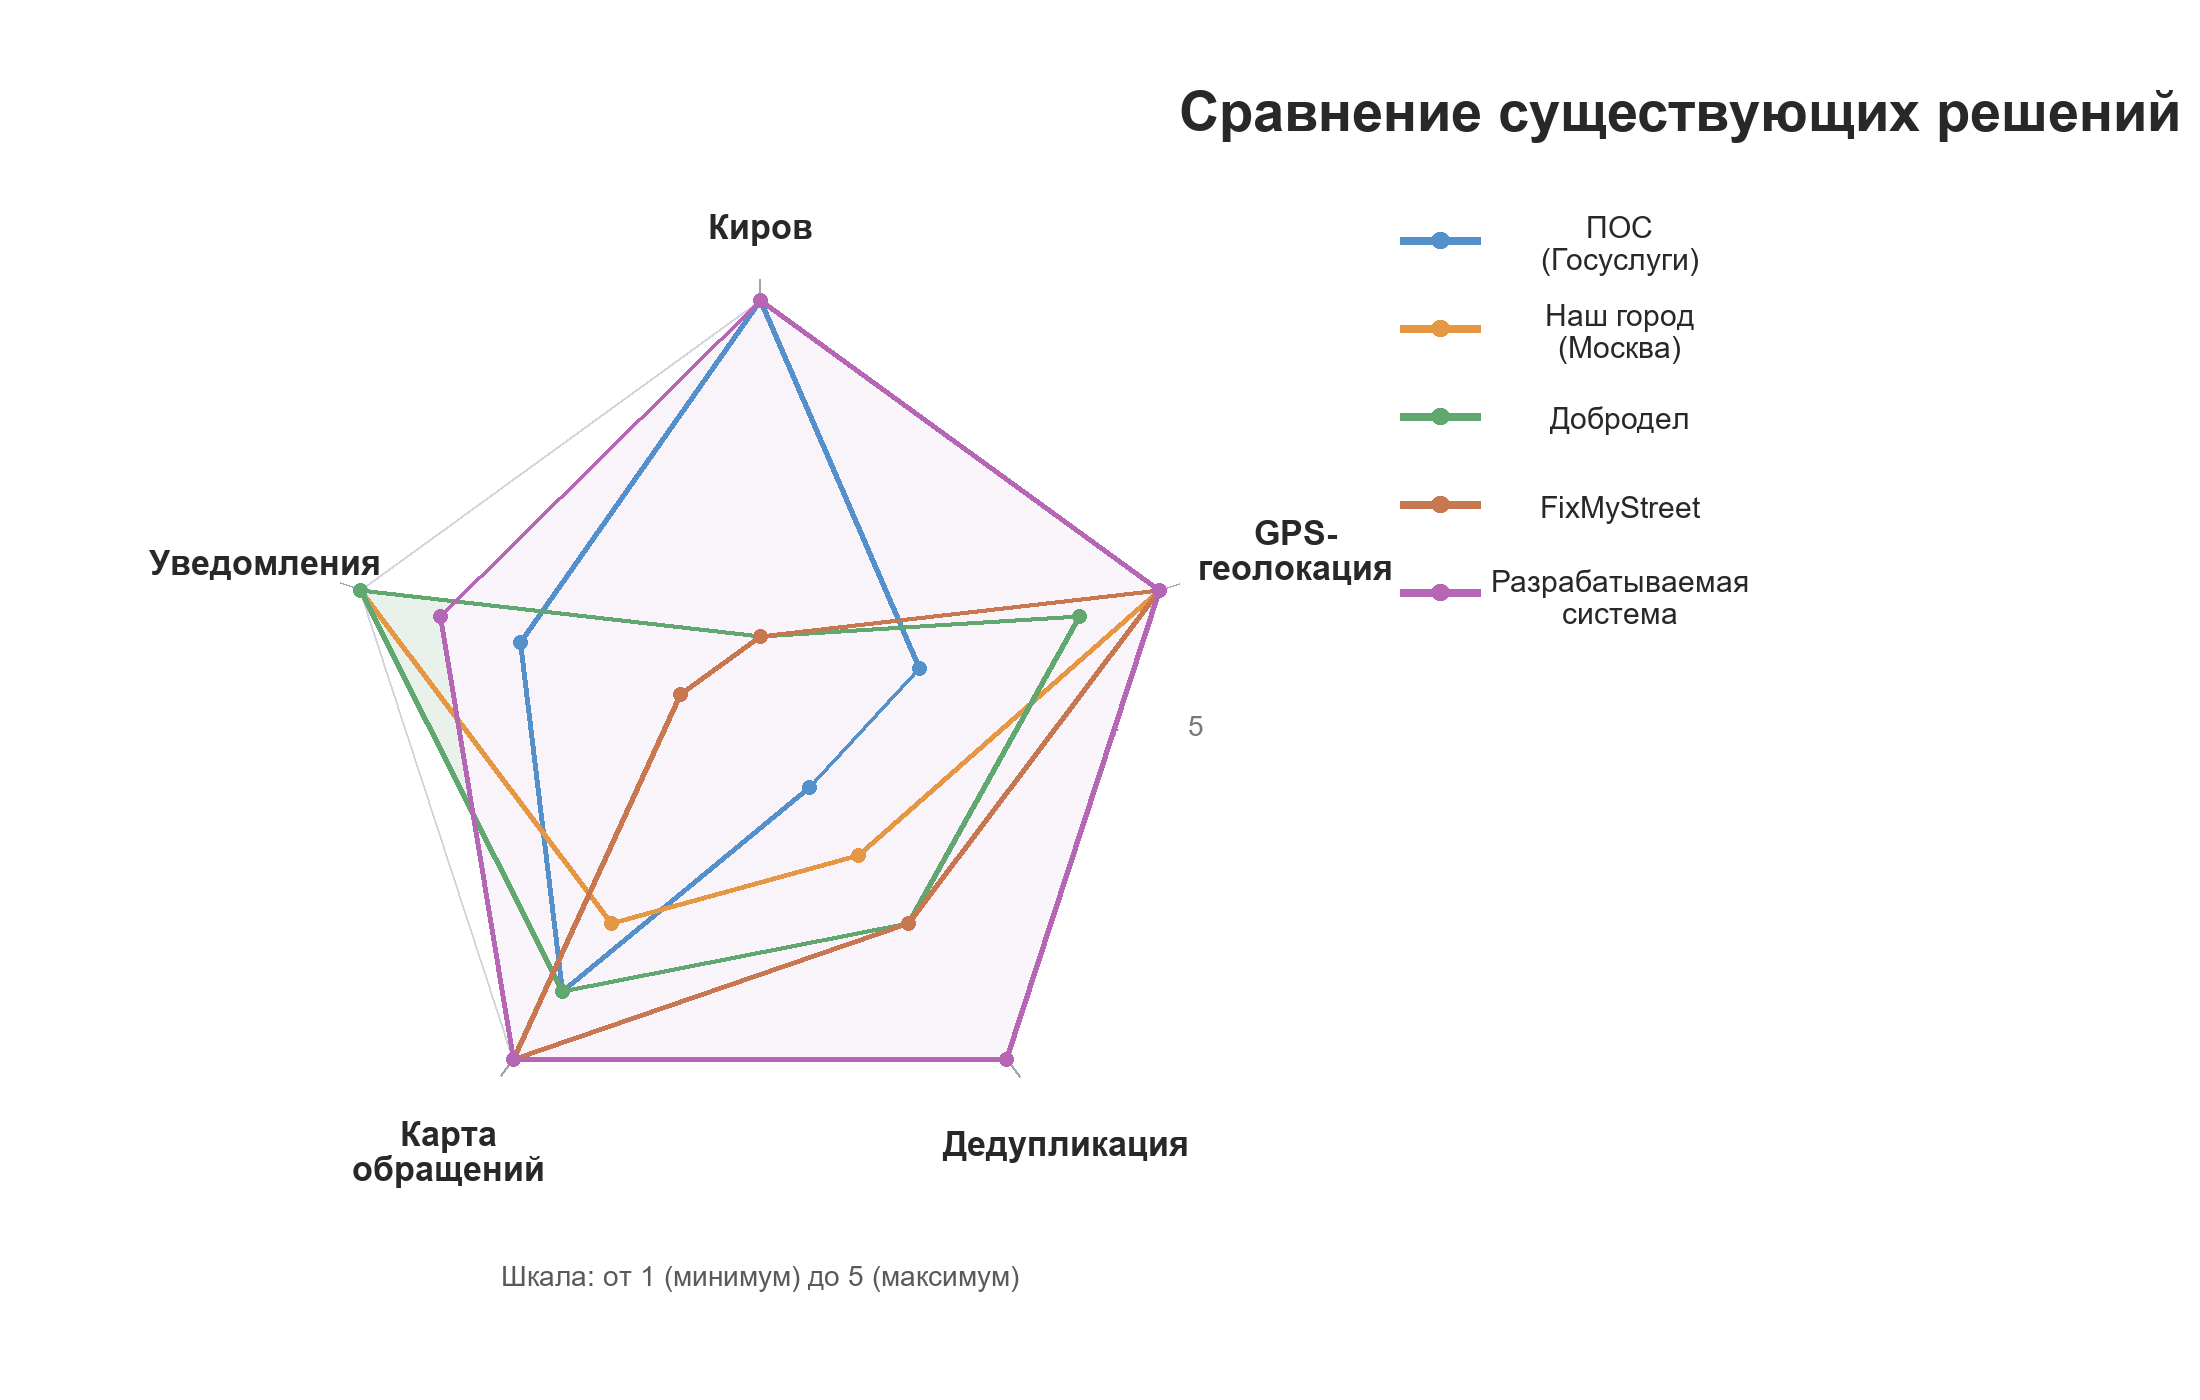
\includegraphics[width=\linewidth,height=0.84\textheight,keepaspectratio]{analogs-radar.png}
\end{frame}

% ========== Слайд 5: Технологический стек ==========
\begin{frame}[c]{Технологический стек}
    \begin{columns}[c,totalwidth=\textwidth]
        \begin{column}{0.2\textwidth}
            \centering
            
\includegraphics[width=\linewidth,height=0.3\textheight,keepaspectratio]{csharp.png}
        \end{column}
        \begin{column}{0.2\textwidth}
            \centering
            
\includegraphics[width=\linewidth,height=0.3\textheight,keepaspectratio]{postgre.png}
        \end{column}
        \begin{column}{0.2\textwidth}
            \centering
            
\includegraphics[width=\linewidth,height=0.3\textheight,keepaspectratio]{react.png}
        \end{column}
        \begin{column}{0.2\textwidth}
            \centering
            
\includegraphics[width=\linewidth,height=0.3\textheight,keepaspectratio]{react_native.png}
        \end{column}
        \begin{column}{0.2\textwidth}
            \centering
            
\includegraphics[width=\linewidth,height=0.3\textheight,keepaspectratio]{expo.png}
        \end{column}
    \end{columns}
    \vfill
    \centering
    \begin{minipage}{0.92\textwidth}
        \centering
        \fontsize{15}{18}\selectfont
        ASP.NET Core + PostgreSQL/PostGIS \quad|\quad React + Яндекс.Карты\\[0.3em]
        React Native + Expo \quad|\quad TypeScript
    \end{minipage}
    \vfill
\end{frame}

% ========== Слайд 6: Структура системы ==========
\begin{frame}[c]{Структура системы}
    \centering
    \vspace{-0.2em}
    \includegraphics[width=\linewidth,height=0.9\textheight,keepaspectratio]{architecture.png}
\end{frame}

% ========== Слайд 7: Структура базы данных ==========
\begin{frame}[c]{Особенности проектирования базы данных}
    \centering
    \vspace{-0.2em}
    \includegraphics[width=\linewidth,height=0.9\textheight,keepaspectratio]{erd-smartcity.png}
\end{frame}

% ========== Слайд 8: Дашборд диспетчера ==========
\begin{frame}[c]{Реализация: дашборд диспетчера}
    \begin{columns}[c,totalwidth=\textwidth]
        \begin{column}{0.34\textwidth}
            \footnotesize
            \begin{itemize}\setlength\itemsep{0.45em}
                \item сводные показатели по обращениям и их статусам;
                \item графики динамики поступления и распределения по категориям;
                \item таблица последних обращений с быстрым переходом к карточке.
            \end{itemize}
        \end{column}
        \begin{column}{0.66\textwidth}
            \centering
            \includegraphics[width=\linewidth,height=0.72\textheight,keepaspectratio]{impl-dashboard.png}
        \end{column}
    \end{columns}
\end{frame}

% ========== Слайд 9: Карта диспетчера ==========
\begin{frame}[c]{Реализация: интерактивная карта диспетчера}
    \begin{columns}[c,totalwidth=\textwidth]
        \begin{column}{0.34\textwidth}
            \footnotesize
            \begin{itemize}\setlength\itemsep{0.45em}
                \item маркеры обращений с цветовой индикацией статуса;
                \item фильтры по состояниям и поиск по карте;
                \item всплывающая карточка выбранного обращения.
            \end{itemize}
        \end{column}
        \begin{column}{0.66\textwidth}
            \centering
            \includegraphics[width=\linewidth,height=0.72\textheight,keepaspectratio]{impl-map.png}
        \end{column}
    \end{columns}
\end{frame}

% ========== Слайд 10: Список обращений (веб) ==========
\begin{frame}[c]{Реализация: список обращений}
    \begin{columns}[c,totalwidth=\textwidth]
        \begin{column}{0.34\textwidth}
            \footnotesize
            \begin{itemize}\setlength\itemsep{0.45em}
                \item табличный перечень обращений с основными полями;
                \item вкладки и поиск для быстрого отбора записей;
                \item переход к детальной карточке по выбору строки.
            \end{itemize}
        \end{column}
        \begin{column}{0.66\textwidth}
            \centering
            \includegraphics[width=\linewidth,height=0.72\textheight,keepaspectratio]{impl-reports.png}
        \end{column}
    \end{columns}
\end{frame}

% ========== Слайд 11: Карточка обращения (веб) ==========
\begin{frame}[c]{Реализация: карточка обращения}
    \begin{columns}[c,totalwidth=\textwidth]
        \begin{column}{0.34\textwidth}
            \footnotesize
            \begin{itemize}\setlength\itemsep{0.45em}
                \item полные данные обращения и история его состояния;
                \item форма смены статуса с комментариями диспетчера;
                \item мини-карта и контактные данные ответственной службы.
            \end{itemize}
        \end{column}
        \begin{column}{0.66\textwidth}
            \centering
            \includegraphics[width=\linewidth,height=0.72\textheight,keepaspectratio]{impl-report-card.png}
        \end{column}
    \end{columns}
\end{frame}

% ========== Слайд 12: Мобильное — создание обращения ==========
\begin{frame}[c]{Мобильное приложение: создание обращения}
    \begin{columns}[c,totalwidth=\textwidth]
        \begin{column}{0.25\textwidth}
            \footnotesize
            \begin{itemize}\setlength\itemsep{0.4em}
                \item Категория, описание и фото с камеры.
                \item Автоопределение GPS или ручной выбор на карте.
                \item Дедупликация в радиусе 50~м.
            \end{itemize}
        \end{column}
        \begin{column}{0.75\textwidth}
            \centering
            \includegraphics[height=0.78\textheight,keepaspectratio]{mobile-create-report-screen.png}
        \end{column}
    \end{columns}
\end{frame}

% ========== Слайд 13: Мобильное — карта ==========
\begin{frame}[c]{Мобильное приложение: карта обращений}
    \begin{columns}[c,totalwidth=\textwidth]
        \begin{column}{0.25\textwidth}
            \footnotesize
            \begin{itemize}\setlength\itemsep{0.4em}
                \item Маркеры с цветовой индикацией статуса.
                \item Фильтры по категориям.
                \item Кнопка геолокации и FAB создания обращения.
            \end{itemize}
        \end{column}
        \begin{column}{0.75\textwidth}
            \centering
            \includegraphics[height=0.78\textheight,keepaspectratio]{mobile-map-screen.png}
        \end{column}
    \end{columns}
\end{frame}

% ========== Слайд 14: Мобильное — список и карточка ==========
\begin{frame}[c]{Мобильное приложение: список и карточка обращений}
    \begin{columns}[c,totalwidth=\textwidth]
        \begin{column}{0.5\textwidth}
            \centering
            \includegraphics[height=0.74\textheight,keepaspectratio]{mobile-reports-list-screen.png}\\
            {\footnotesize Список обращений}
        \end{column}
        \begin{column}{0.5\textwidth}
            \centering
            \includegraphics[height=0.74\textheight,keepaspectratio]{mobile-report-detail-screen.png}\\
            {\footnotesize Карточка обращения}
        \end{column}
    \end{columns}
\end{frame}

% ========== Слайд 15: Тестирование ==========
\begin{frame}[c]{Тестирование}
    \begin{columns}[c,totalwidth=\textwidth]
        \begin{column}{0.35\textwidth}
            \footnotesize
            \begin{itemize}\setlength\itemsep{0.4em}
                \item Модульные и интеграционные тесты серверной части (xUnit).
                \item Модульные тесты мобильного приложения (Vitest, 20 тестовых файлов).
                \item Тестирование API через Swagger~UI.
                \item Функциональное тестирование веб-панели.
            \end{itemize}
        \end{column}
        \begin{column}{0.65\textwidth}
            \centering
            \includegraphics[width=\linewidth,height=0.72\textheight,keepaspectratio]{tests-runner-result.png}
        \end{column}
    \end{columns}
\end{frame}

% ========== Слайд 16: Перспективы развития ==========
\begin{frame}[c]{Перспективы развития}
    \begin{itemize}\setlength\itemsep{0.5em}
        \item внедрение push-уведомлений на уровне операционной системы;
        \item расширение возможностей работы при нестабильном сетевом соединении;
        \item развитие функциональности модуля городских событий;
        \item интеграция с внешними картографическими сервисами для обратного геокодирования;
        \item реализация ролевой модели с несколькими уровнями доступа для диспетчеров.
    \end{itemize}
\end{frame}

% ========== Слайд 17: Заключение ==========
\begin{frame}[c]{Заключение}
    \centering
    \Large
    Все поставленные задачи выполнены.\\[0.6cm]
    Разработанная программная система готова к дальнейшему развитию.\\[0.6cm]
    Спасибо за внимание!
\end{frame}

\end{document}
